\chapter{Experimental Setups}
\label{sec:experiment}

To experiment with different solutions for sentiment analysis, a system testing platform and code base was developed. This testing system generates and trains different models based on input arguments as default values for algorithms and type of algorithm. The architecture and flow of this system is described as a part of section~\ref{sec:classifier_arch}.

The testing system can take in a set of parameters to use for an algorithm, like pre-processor methods, whether or not to use inverse document frequency (\nom{IDF}{Inverse Document Frequency}) or stop words, and so on, or a grid search flag can be set. If the grid search option is activated, a model is generated with the best possible parameters set for the given algorithm. The grid search is conducted using k-fold cross validation, and the set of parameters to search across. The parameter search space is reflected in table~\ref{tab:gridsearch_params}. The following parameters were included in the search. Three binary ($Yes$/$No$) parameters: $Use IDF$, $Use Smooth IDF$, and $Use Sublinear IDF$, together with $ngram$ ($unigram$/$bigram$/$trigram$). SVM and MaxEnt models in addition included $C$ and NB models $alpha$ parameters, all with the value ranges [$0.1/0.3/0.5/0.7/0.8/1.0$]. MaxEnt models also had \textit{penalty} ($L1$/$L2$).


\begin{table}[t!]
\centering
\begin{tabular}{|r||c|c|c|} 
\cline{2-4}

\multicolumn{1}{c|}{ } & \textbf{NB} & \textbf{SVM} & \textbf{MaxEnt} \\ \hline

penalty  &  - &  - & L1 or L2 \\ \hline
alpha/C  & \multicolumn{3}{ c| }{<0.1, 0.3, 0.5, 0.7, 0.8, 1.0>} \\ \hline
ngram &  \multicolumn{3}{ c| }{ Unigram, Bigram or Trigram } \\ \hline
Remove Stop Words &  \multicolumn{3}{ c| }{ Yes or No } \\ \hline
Use IDF &  \multicolumn{3}{ c| }{ Yes or No } \\ \hline
Use Smooth IDF &  \multicolumn{3}{ c| }{ Yes or No } \\ \hline
Use Sublinear IDF &  \multicolumn{3}{ c| }{ Yes or No } \\ \hline

\end{tabular}
\caption{Overview of parameter search space for the grid searches conducted in the experiments.}
\label{tab:gridsearch_params}
\end{table}


\section{Pre-processing and Feature Selection}

This section describes the different pre-processing implementations used; what placeholders, negation attachment and reducing letter duplications is.

To find the best features to use and what kind of pre-processing was the best, a set of 8 different combinations of pre-processing methods was designed. The different methods include no pre-processing, where all characters are included as features; full remove where all special Twitter features like user names, URLs, hash tags and emoticons are stripped; and one where the Twitter features are replaced with placeholder texts to reduce vocabulary. A full overview of the pre-processing methods is given in~table~\ref{tab:preproc_desc}.

\begin{table}[t!]
	\centering
	\begin{tabular}{|r||c|c|c|c|c|c|c|c|}
		% P1  -> no\_usernames
		% P2 -> remove\_noise
		% P3 -> placeholders
		% P4 -> all
		% P5 -> remove\_all
		% P6 -> reduced\_attached
		% P7 -> no\_url\_usernames \_reduced \_attached

		\cline{2-9}
	 \multicolumn{1}{c| }{ } & \textbf{None} & \textbf{P1} & \textbf{P2} & \textbf{P3} & \textbf{P4} & \textbf{P5} & \textbf{P6} & \textbf{P7}  \\ \hline
%	 Remove Usernames                     & & x & x &   & x & x & & x \\ \hline
%	 		$||U||$ instead of $@username$       & &   &   & x &   &   & & \\ \hline
%	 		Remove URLs                          & &   & x &   & x & x & & x \\ \hline
%	 		$||URL||$ instead of real URL        & &   &   & x &   &   & & \\ \hline
%	 		Remove Hash-tags                     & &   &   &   & x & x & & \\ \hline
%	 		Hash-tags as words                   & &   & x &   &   &   & & \\ \hline
%	 		$||H||$ instead of hash-tag          & &   &   & x &   &   & & \\ \hline
%	 		Remove $RT$-tag                      & &   & x &   & x & x & & \\ \hline
%	 		Remove emoticons                     & &   &   &   & x & x & & \\ \hline
%	 		Reduce letter duplicates             & &   & x &   & x &   & x & x \\ \hline
%	 		Attach negation to surrounding words & &   &   &   & x &   & x & x \\ \hline
	 
	 
		Remove Usernames                     & & x & x &   & x & x & & x \\ \hline
		Username placeholder       & &   &   & x &   &   & & \\ \hline
		Remove URLs                          & &   & x &   & x & x & & x \\ \hline
		URL placeholder        & &   &   & x &   &   & & \\ \hline
		Remove Hash-tags                     & &   &   &   & x & x & & \\ \hline
		Hash-tags as words                   & &   & x &   &   &   & & \\ \hline
		Hash-tag placeholder          & &   &   & x &   &   & & \\ \hline
		Remove $RT$-tag                      & &   & x &   & x & x & & \\ \hline
		Remove emoticons                     & &   &   &   & x & x & & \\ \hline
		Reduce letter duplicates             & &   & x &   & x &   & x & x \\ \hline
		Attach negation  & &   &   &   & x &   & x & x \\ \hline
	\end{tabular}
	\caption[Description of used pre-processing methods]{Description of the pre-processing methods used for the experiments. Some functions remove entities, other replace them with a placeholder text. The hash-tag as word transforms a hash-tag to a regular word and uses the hash-tag as a feature. "Reduce letter duplicates", reduces redundant letters to a maximum of three.}
	\label{tab:preproc_desc}
\end{table}

\subsection{Removing features}
To reduce the vocabulary and to get more precise classification, some features were omitted. User names are most likely to be considered noisy, but in some cases they may be relevant for a text's sentiment. The same goes for URLs, \nom{RT}{Re-Tweet}-tags and emoticons. Some methods, like P1, P2, P4, P5 and P7 consider the user names noisy and remove them from the text. Removing features will remove all notion of the feature, unlike when replacing it with a placeholder.

\subsection{Replacing with placeholders}
There might be a chance that URLs or user names are relevant for the sentiment. Not necessarily the value of the name or URL itself, but the fact that there are references to URLs and user names. To make these features more informative for the machine learning algorithms, a pre-processing method (P3) was implemented for replacing them with placeholder texts. This means that a user name like $@$$someuser$ is replaced by the text $||U||$. $||U||$ was chosen as it is very unlikely that it would be a part of the original tweet. Hash-tags ($\#hash$) are replaced by $||H||$ and URLs by $||URL||$. 

\subsection{Reducing letter duplication}
By reducing and normalizing excessive letter duplications like "I'm sooo-ooo happyyyyyyyy!!!!!!", the vocabulary is reduced and the classification can perform better. However, there might be that the word "sooooo" is more sentimentally charged than the proper form of the word "so". The sentence "I'm sooooooo happyyyyyyyy!!!!!!" is more positive polar than the statement "I'm so happy!".

To reduce the vocabulary but not lose information, all duplicates of more than three consecutive characters are reduced to exactly three duplications. So "I'm sooooooo happyyyyyyyy!!!!!!" would be changed to "I'm sooo happyyy!!!", and the same goes for "I'm sooooooooooooooo happyyyyyyyy!!!!!!". This way the additional sentiment is preserved.

\subsection{Attaching negation}

The negation word "not" can change the polarity of an entire sentence. The sentence "I am happy" is obviously positive, and "I am not happy" negative. If using unigrams, the features of the second sentence would have been $('I', 'am', 'not', 'happy')$ and for the first one $('I', 'am', 'happy')$. Both having the word "happy" in them, and if that were to be a significant feature for positive classification, the negative sentence could be classified as positive.

By attaching the negation word to the preceding and the following word, the features will also reflect the change in polarity. So the features for the negative sentence would be $('I', 'am-not', 'not-happy')$.

\section{SemEval'13}

The system from this Master's Thesis participated in a workshop with focus on semantic analysis systems. SemEval'13\footnote{\url{http://www.cs.york.ac.uk/semeval-2013/}} had several shared tasks, but we only took part in Task 2B; building a message polarity classification system in Twitter. The task had two parts: unconstrained and constrained systems. The unconstrained system allowed for a training set in addition to the one provided by SemEval'13, while the constrained system could only use the provided set. To test the systems beyond Twitter, SemEval'13 also evaluated the systems using a Short Message (or Messaging) Service~(\nom{SMS}{Short Message (or Messaging) Service}) test set. Thus, there were a total of four different deliveries to SemEval'13: Twitter unconstrained and constrained, and SMS unconstrained and constrained.

\section{Visualisation Applications}

To test the visualisation applications, an experiment to predict the outcome of the Eurovision Song Contest~(\nom{ESC}{Eurovision Song Contest}) was conducted.

Eurovision Song Contest is a popular annual cross-Europe song contest. Each country participates with their selected song, and every country vote for their favourite song to win the contest. A country cannot vote on their own song. In addition to tele-voting in each country, a country also has a panel of judges giving expert opinions.

ESC has historically been criticized for being too political, but research can indicate otherwise. \cite{ginsburgh2008eurovision} show that the amount of vote trading is rather minimal and that the voting is more cultural and geographical than political. Furthermore, \cite{ginsburgh2008eurovision} suggest that immigration can have some impact on voting. In any case, it may be plausible that the amount of tele-voters for ESC is equal to the amount of people tweeting about a given country contribution.

To predict the outfall of ESC, the SentiStack application was used. This allows for several Twitter Search queries to be compared to each other, and thus see what may be considered as favourites. The predictions were carried out before the ESC final, but after the semi-finals.  

%\subsubsection{SentiMap After a Natural Disaster}
%
%After the Oklahoma Tornado disaster\footnote{2013 Moore tornado: \url{http://en.wikipedia.org/wiki/2013_Moore_tornado}}, the experiment executed was to observe the SentiMap application, and see how the natural disaster affected the sentiment across the nation. 


\chapter{Results}
\label{sec:results}


The experimental results is split into four different sections. In the first section, the full grid search results are defined. In the second, a detailed comparison of the best algorithms can be found. Section~\ref{sec:semeval_result} describes the result from SemEval'13, and~Section~\ref{sec:esc_result} covers the ESC experiment.

\section{Full Grid Search}

As described above, an extensive grid search was conducted. This search cycled through different algorithms, parameters and preprocessing techniques. Figure~\ref{fig:results_full} displays the precision, recall, F1-score and accuracy for each of the classifiers with dev 1 as evaluation data. We notice that most of the classifiers that involve the NB algorithm have a bad performance, both for accuracy and F1-score. Further, we can see that the MaxEnt classifier has the best accuracy, while SVM has a slightly better F1-score.

Two-step models with SVM-based subjectivity classification exhibit the same basic behaviour. The one-step MaxEnt model classifies more tweets as neutral than the other classifiers. Using MaxEnt for subjectivity classification and either MaxEnt or SVM for polarity classification performs well, but is too heavy on the positive class. Boosting does not improve and behaves in a fashion similar to two-step MaxEnt models. All combinations involving NB tend to heavily favour positive predictions; only the two-step models involving another algorithm for polarity classification gave some improvement for negative tweets.

We can also see that all the classifiers with SVM tend to give a better confusion matrix than the others. This is shown in Figures~\ref{fig:confmat_svm} - \ref{fig:confmat_boosting}. The figures show what classifications that were correct. The columns are [$negative$, $neutral$, $positive$]. This means that the top left box is how many tweets that were classified as negative, and actually were negative, the box to the left is how many tweets were classified as neutral, but was negative. The blue colour indicate low number of tweets, and the red colour indicate a high number. What we would like to see is a red colour on the diagonal. The confusion matrices that include SVM indicate that it has a more precise classification of negative instances than the others. In tests where NB is used, the system leans much more to the positive class than the other models.

As a part of the grid search, the system applied all the different preprocessing methods for each classifier. Figure~\ref{fig:preprocess_usage} shows that $P2$ (removing user names, URLs, hash- tags prefixes, retweet tokens, and redundant letters) is the preprocessing method which performs best (gives the best accuracy) and thus used most often (10 times). Figure~\ref{fig:preprocess_usage} also indicates that URLs are noisy and do not contain much sentiment, while hashtags and emoticons tend to be more valuable features ($P2$ and $P7$ \textemdash~removing URLs \textemdash~perform best, while $P4$ and $P5$ \textemdash~removing hashtags and emoticons in addition to URLs \textemdash~perform badly).

\begin{sidewaysfigure}[tb!]
 \begin{center}
     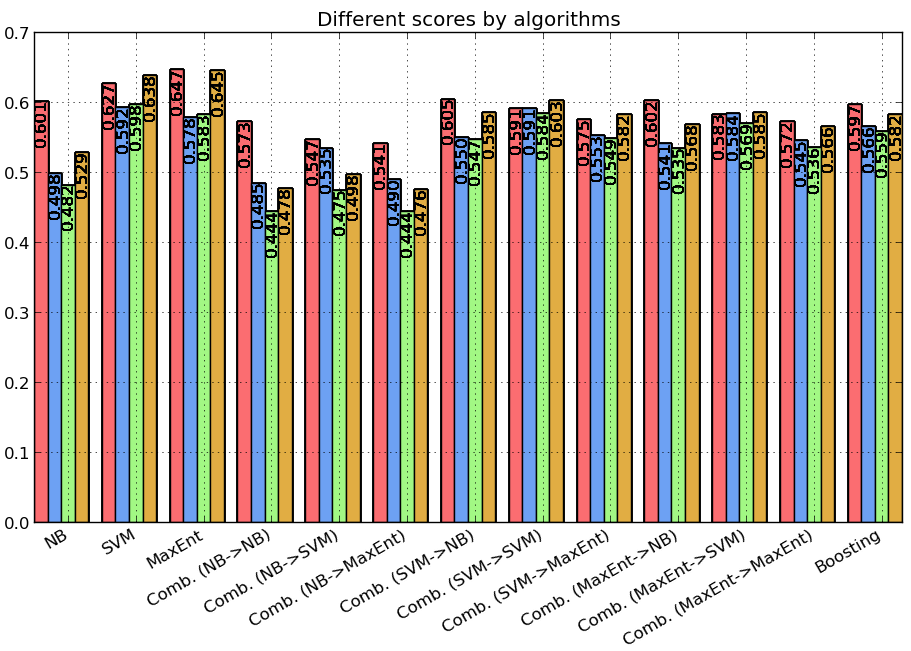
\includegraphics[width=\linewidth]{../img/plots/grid/full_biggersize.png}
 \end{center}
 \caption[Results overview across all models]{A full overview of the performance of the different models after a full grid search. Two models stand out as having highest accuracies: SVM and MaxEnt. One can also see that models using Na\"{i}ve Bayes, especially on its own or to classify subjectivity, perform poorly.}
 \label{fig:results_full}
\end{sidewaysfigure}

\clearpage

\begin{minipage}[t!]{\linewidth}
     \centering
     \begin{minipage}{0.45\linewidth}
          \begin{figure}[H]
               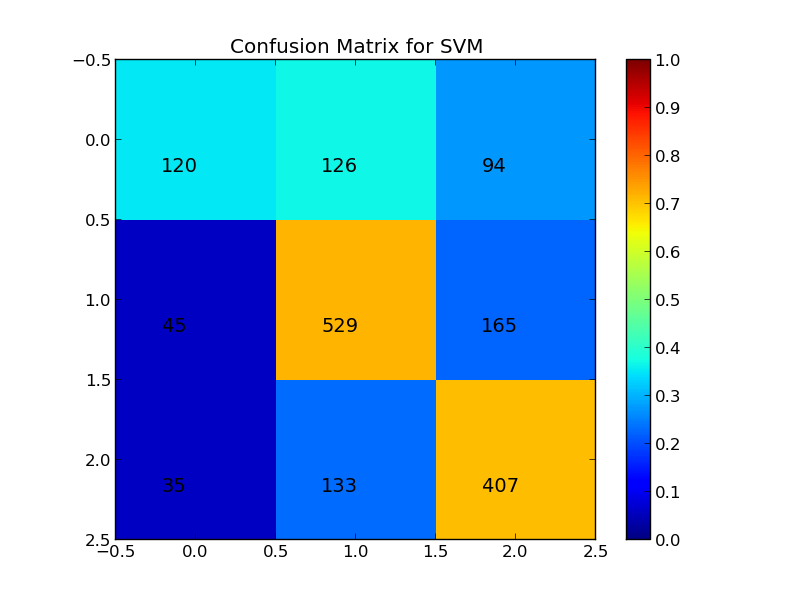
\includegraphics[width=\linewidth]{../img/plots/grid/confusion_matrix_SVM.png}
           \caption[The confusion matrix for SVM]{Confusion matrix for the model using SVM. Performs well on both neutral and positive predictions, but somewhat poorly on negative.}
           \label{fig:confmat_svm}
          \end{figure}
     \end{minipage}
     \hspace{0.05\linewidth}
     \begin{minipage}{0.45\linewidth}
          \begin{figure}[H]
               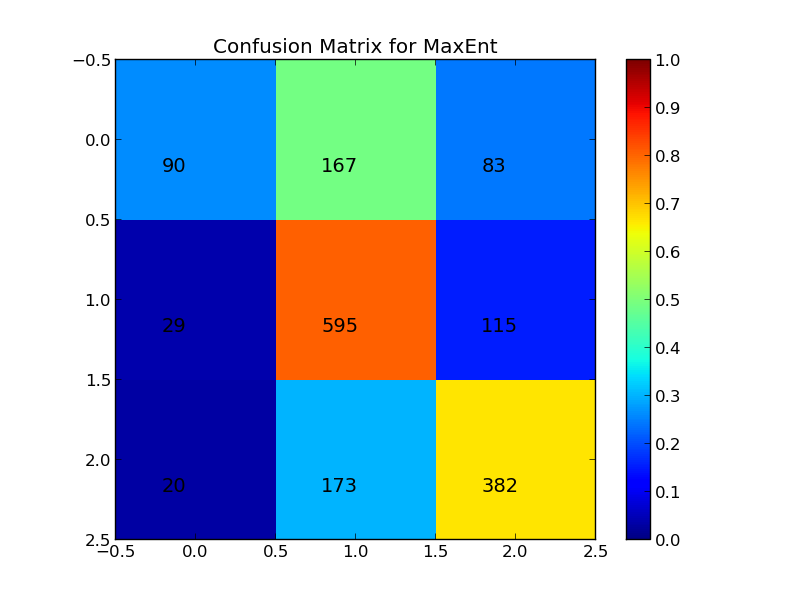
\includegraphics[width=\linewidth]{../img/plots/grid/confusion_matrix_MaxEnt.png}
           \caption[The confusion matrix for MaxEnt]{Confusion matrix for the model using MaxEnt. Performs especially good on neutral tweets, but seems to be classifying neutral too much.}
           \label{fig:confmat_maxent}
          \end{figure}
     \end{minipage}
     \begin{minipage}{0.45\linewidth}
          \begin{figure}[H]
               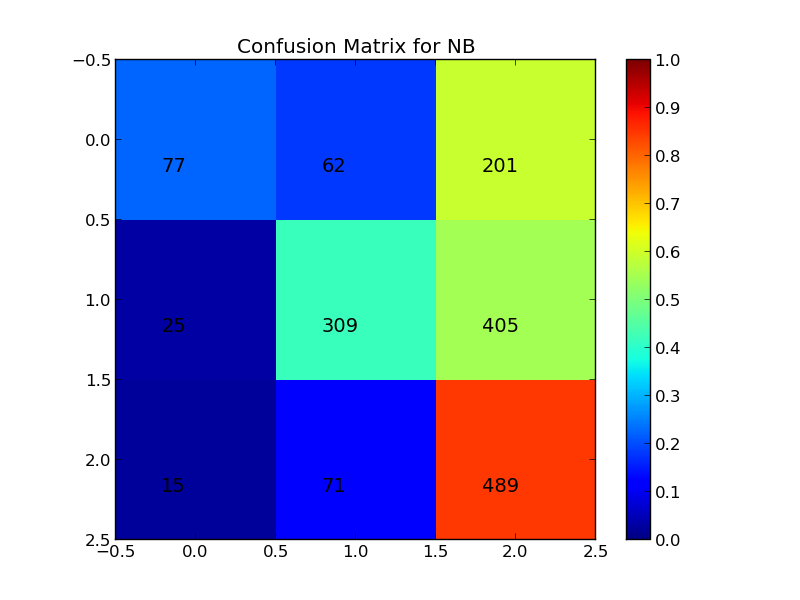
\includegraphics[width=\linewidth]{../img/plots/grid/confusion_matrix_NB.png}
           \caption[The confusion matrix for NB]{Confusion matrix for the model using NB. Performs very well for positive tweets, but seems to favour them too much.}
           \label{fig:confmat_nb}
          \end{figure}
     \end{minipage}
     \hspace{0.05\linewidth}
     \begin{minipage}{0.45\linewidth}
          \begin{figure}[H]
               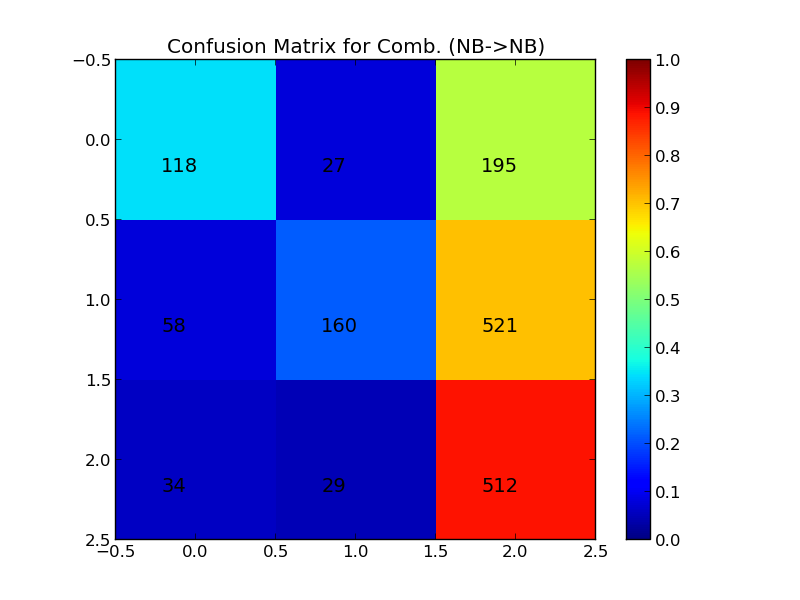
\includegraphics[width=\linewidth]{../img/plots/grid/confusion_matrix_Comb-NB-NB.png}
           \caption[The confusion matrix for two-step NB -> NB]{Confusion matrix for the two-step model using NB for both subjectivity/objectivity and polarity classification. Shows the same trend as when using NB in a one-step model: the model favours positive predictions.}
           \label{fig:confmat_nb_nb}
          \end{figure}
     \end{minipage}
\end{minipage}

\begin{minipage}[t!]{\linewidth}
     \centering
     \begin{minipage}{0.45\linewidth}
          \begin{figure}[H]
               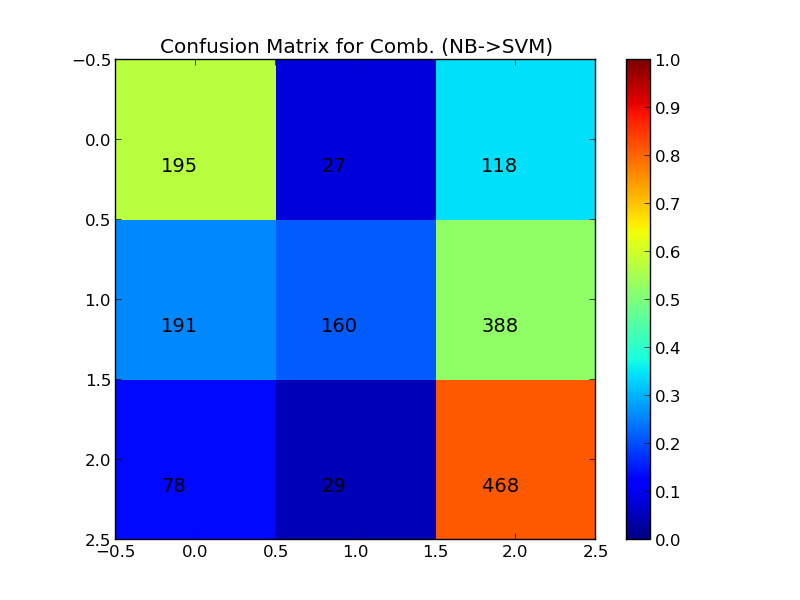
\includegraphics[width=\linewidth]{../img/plots/grid/confusion_matrix_Comb-NB-SVM.png}
           \caption[The confusion matrix for two-step NB -> SVM]{Confusion matrix for the two-step model using NB for subjectivity/objectivity classification and SVM for polarity. Shows the same trend as when using NB in a one-step model: the model favours positive predictions but is performing better for negative tweets.}
           \label{fig:confmat_nb_svm}
          \end{figure}
     \end{minipage}
     \hspace{0.05\linewidth}
     \begin{minipage}{0.45\linewidth}
          \begin{figure}[H]
               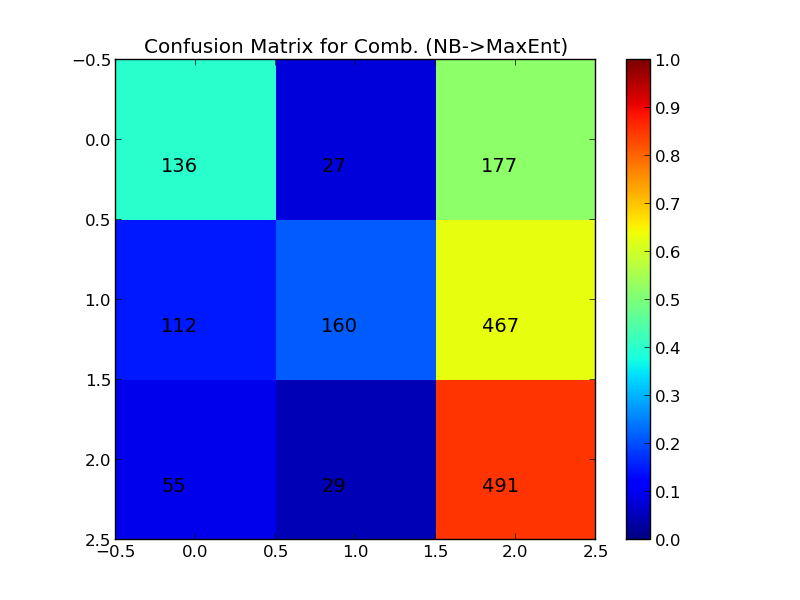
\includegraphics[width=\linewidth]{../img/plots/grid/confusion_matrix_Comb-NB-MaxEnt.png}
           \caption[The confusion matrix for two-step NB -> MaxEnt]{Confusion matrix for the two-step model using NB for subjectivity/objectivity classification and SVM for polarity. Shows the same trend as when using the NB -> SVM model: the model favours positive predictions but is performing better for negative tweets.}
           \label{fig:confmat_nb_maxent}
          \end{figure}
     \end{minipage}
\end{minipage}

\begin{minipage}[t!]{\linewidth}
     \centering
     \begin{minipage}{0.45\linewidth}
           \begin{figure}[H]
                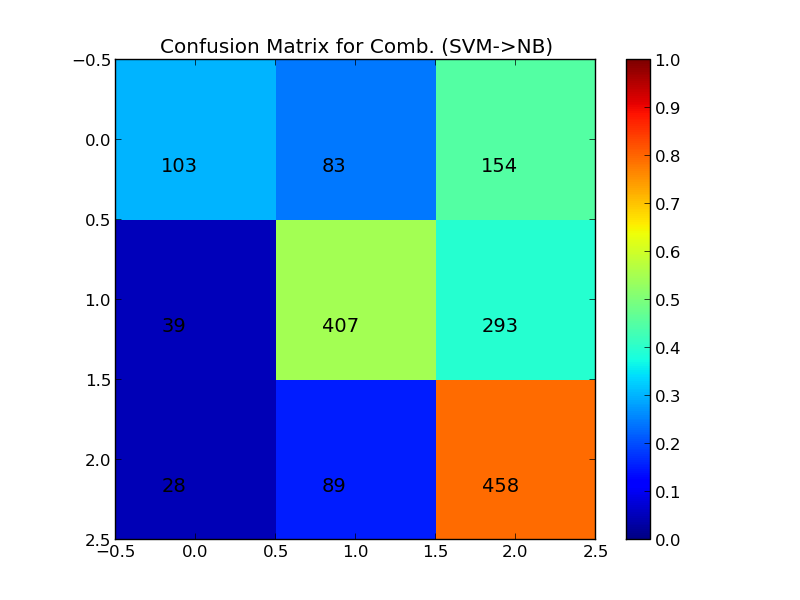
\includegraphics[width=\linewidth]{../img/plots/grid/confusion_matrix_Comb-SVM-NB.png}
        		\caption[The confusion matrix for two-step SVM -> NB]{Confusion matrix for the model using SVM and NB. Performs well for positive tweets, but not as well for neutral and negative.}
            \label{fig:confmat_svm_nb}
           \end{figure}
      \end{minipage}
      \hspace{0.05\linewidth}
      \begin{minipage}{0.45\linewidth}
           \begin{figure}[H]
                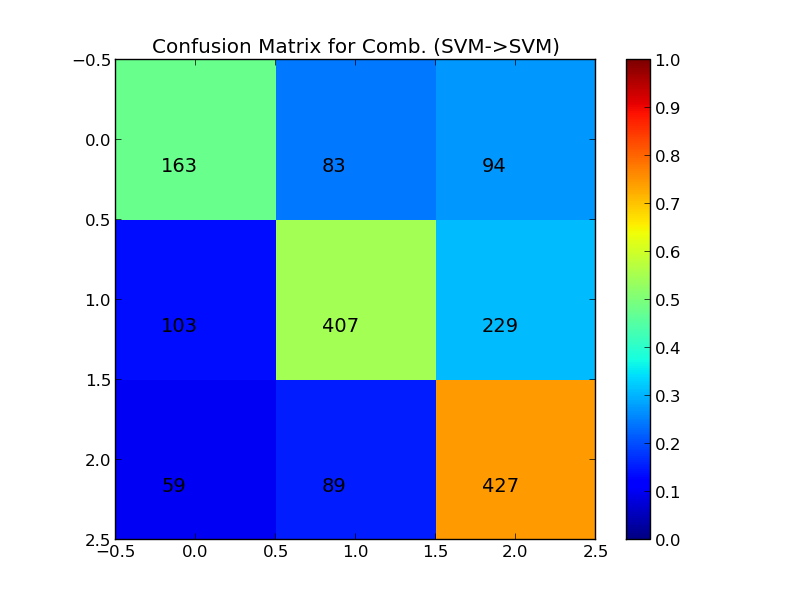
\includegraphics[width=\linewidth]{../img/plots/grid/confusion_matrix_Comb-SVM-SVM.png}
         		\caption[The confusion matrix for two-step SVM -> SVM]{Confusion matrix for the model using SVM and SVM. Performs well across the board, and shows a good diagonal colour profile in the plot.}
            \label{fig:confmat_svm_svm}
           \end{figure}
      \end{minipage} \\
 \end{minipage}
 
 \begin{minipage}[t!]{\linewidth}
      \centering
     \begin{minipage}{0.45\linewidth}
          \begin{figure}[H]
               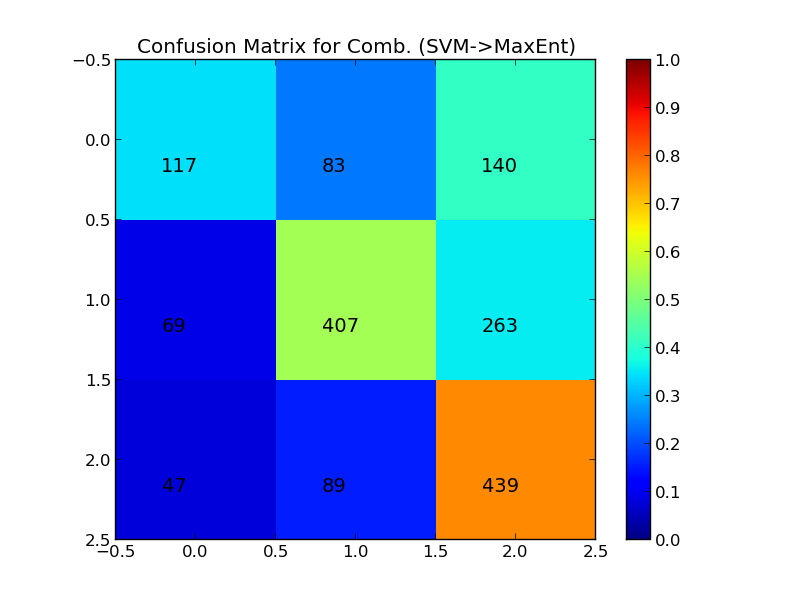
\includegraphics[width=\linewidth]{../img/plots/grid/confusion_matrix_Comb-SVM-MaxEnt.png}
           \caption[The confusion matrix for two-step SVM -> MaxEnt]{Confusion matrix for the model using SVM and MaxEnt. Performs well for neutral and positive tweets, but not too well on negative tweets.}
           \label{fig:confmat_svm_maxent}
          \end{figure}
     \end{minipage}
     \hspace{0.05\linewidth}
     \begin{minipage}{0.45\linewidth}
          \begin{figure}[H]
               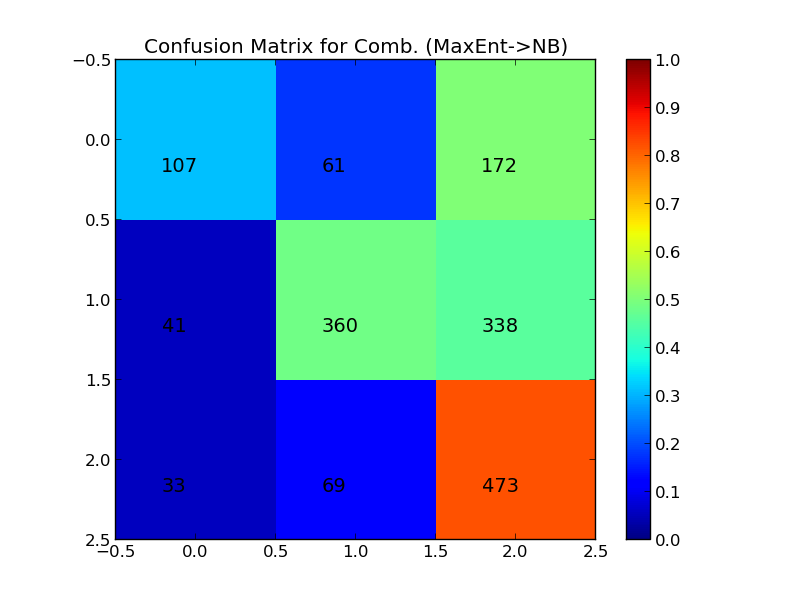
\includegraphics[width=\linewidth]{../img/plots/grid/confusion_matrix_Comb-MaxEnt-NB.png}
           \caption[The confusion matrix for two-step MaxEnt -> NB]{Confusion matrix for the model using MaxEnt and NB. Performs well for positive tweets, but not too well on negative and neutral tweets.}
           \label{fig:confmat_maxent_nb}
          \end{figure}
     \end{minipage}
\end{minipage}
     
\begin{minipage}[t!]{\linewidth}
     \centering
     \begin{minipage}{0.45\linewidth}
          \begin{figure}[H]
               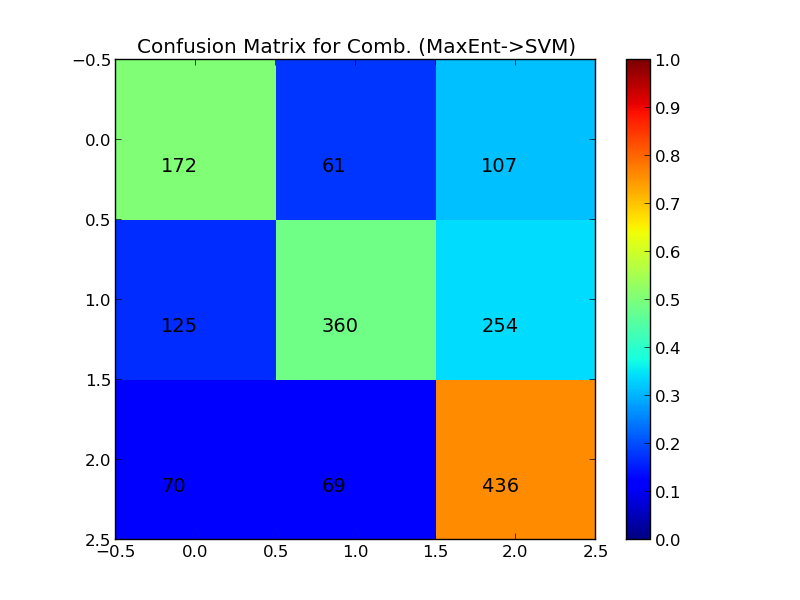
\includegraphics[width=\linewidth]{../img/plots/grid/confusion_matrix_Comb-MaxEnt-SVM.png}
           \caption[The confusion matrix for two-step MaxEnt -> SVM]{Confusion matrix for the model using MaxEnt and SVM. Performs well but is too heavy on the positive classification.}
           \label{fig:confmat_maxent_svm}
          \end{figure}
     \end{minipage}
     \hspace{0.05\linewidth}
     \begin{minipage}{0.45\linewidth}
          \begin{figure}[H]
               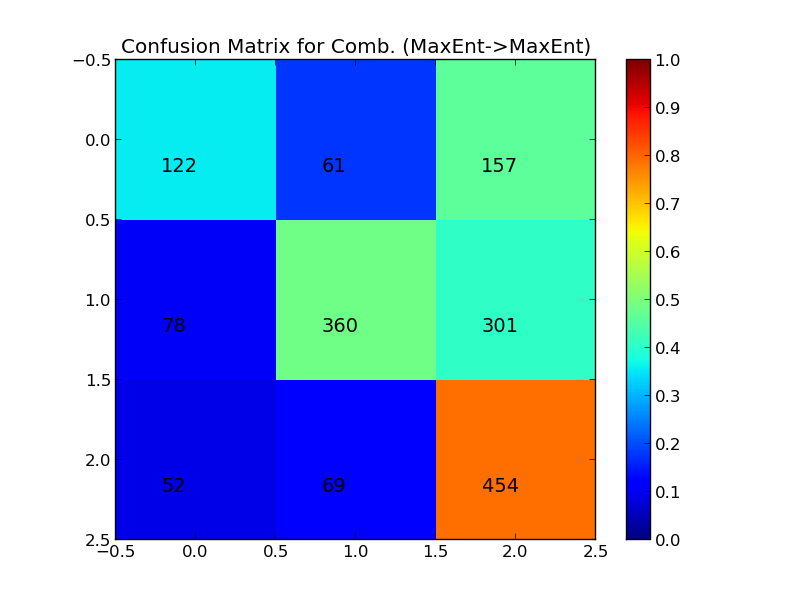
\includegraphics[width=\linewidth]{../img/plots/grid/confusion_matrix_Comb-MaxEnt-MaxEnt.png}
           \caption[The confusion matrix for two-step MaxEnt -> MaxEnt]{Confusion matrix for the model using MaxEnt and MaxEnt. As with MaxEnt -> SVM, this model performs well but is too heavy on the positive classification.}
           \label{fig:confmat_maxent_maxent}
          \end{figure}
     \end{minipage}
\end{minipage}

\begin{minipage}[t!]{\linewidth}
     \centering
     \begin{minipage}{0.45\linewidth}
	     \begin{figure}[H]
	          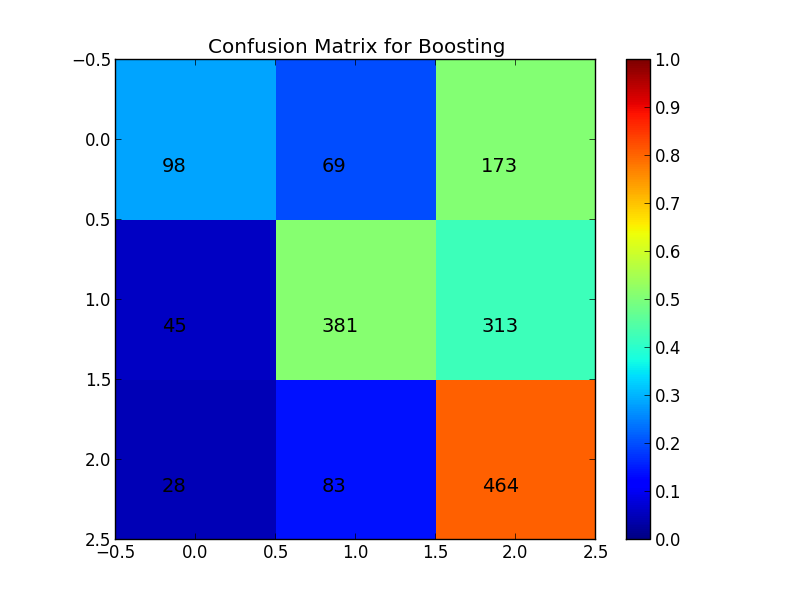
\includegraphics[width=\linewidth]{../img/plots/grid/confusion_matrix_Boosting.png}
	      \caption[The confusion matrix for Boosting]{Confusion matrix for the model using Boosting. Showing the same trend as the MaxEnt -> SVM and MaxEnt -> MaxEnt models: it tends to classify too many tweets as positive.}
	      \label{fig:confmat_boosting}
	     \end{figure}
     \end{minipage}
\end{minipage}

\begin{figure}[b!]
	\centering
	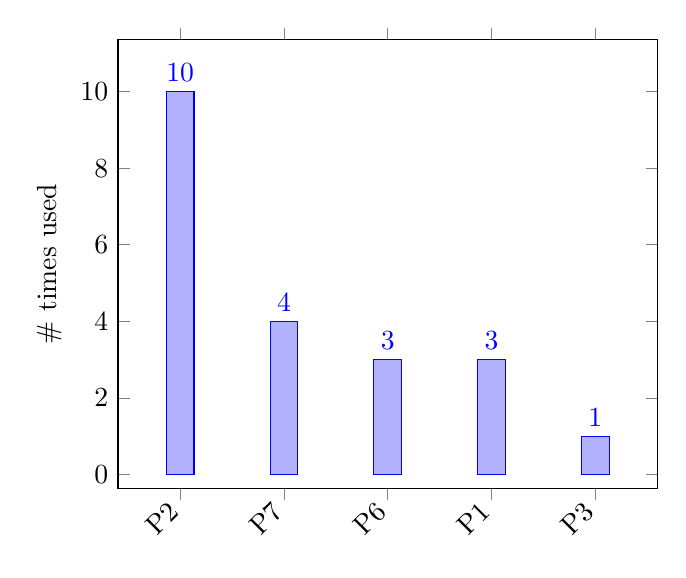
\begin{tikzpicture}
	  \begin{axis}[
	    ybar,
	    enlargelimits=0.15,
	    legend style={at={(0.5,-0.2)},
	      anchor=north,legend columns=-1},
	    ylabel={\# times used},
	    symbolic x coords={P2,P7,P6, P1,P3},
	    xtick=data,
	    nodes near coords, 
		nodes near coords align={vertical},
	    x tick label style={rotate=45,anchor=east},
	    ]
	    \addplot coordinates {(P2,10) (P7,4) 
			(P6,3) (P1,3) (P3,1)};
	  \end{axis}
	\end{tikzpicture}
	\caption[Statistics of pre-processing usage.]{Statistics of pre-processing usage. Removing all usernames, URLs, hash-tag characters, RT-tags and excessive letters seem to give best performance.}
	\label{fig:preprocess_usage}
\end{figure}

\clearpage

\section{SVM vs MaxEnt}

\begin{table}[t!]
\centering
\begin{tabular}{|r||c|c|c|} 
\cline{2-3}
\multicolumn{1}{c|}{ } & \textbf{SVM} & \textbf{MaxEnt} \\ \hline
ngram\_range & 1,1 & 1,1 \\ \hline
sunlinear\_tf  & True & True \\ \hline
preprocessor & P2 & P3 \\ \hline
use\_idf & True & True \\ \hline
smooth\_idf & True & True \\ \hline
max\_df & 0.5 & 0.5 \\ \hline
stop\_words & None & None \\ \hline
C & 1.0 & 0.3 \\ \hline
penalty &  & L1 \\ \hline

\end{tabular}
\caption[Selected parameters from grid search]{The parameters selected for SVM and MaxEnt models through extensive grid search.}
\label{tab:svm_maxent_best_params}
\end{table}

From the full grid search, the best parameters on SVM and MaxEnt were extracted and more detailed tests were carried out only using SVM and MaxEnt, without grid searching. The best parameter setting for the SVM model was using unigram, the $P2$ preprocessing method, not removing stop words, and a $C$ value of $1.0$. For the MaxEnt model, the $P3$ preprocessing method was used, along with unigrams, IDF, not removing stop words, and $0.3$ as $C$ value. The penalty for MaxEnt was selected to be L1. Full parameter selection for SVM and MaxEnt is visible in~table~\ref{tab:svm_maxent_best_params}. The SVM and MaxEnt models, with these parameters, were tested with an additional development set (the data set Dev 2; see table~\ref{tab:datasets}).

The results for both the SVM and MaxEnt classifiers with Dev 1 are shown in figure~\ref{fig:best_result}. With Dev 2, SVM's performance is much better than MaxEnt's, as seen in table~\ref{tab:performance}. Dev 1 contains more neutral tweets than Dev 2, which gives us a reason to believe that it favours the MaxEnt classifier. In MaxEnt's confusion matrix from the first search, shown in Figure~\ref{fig:confmat_maxent}, we can see that it classifies more neutral tweets than the other classifiers.

\begin{figure}[t!]
	\centering
	\begin{minipage}{.45\linewidth}
		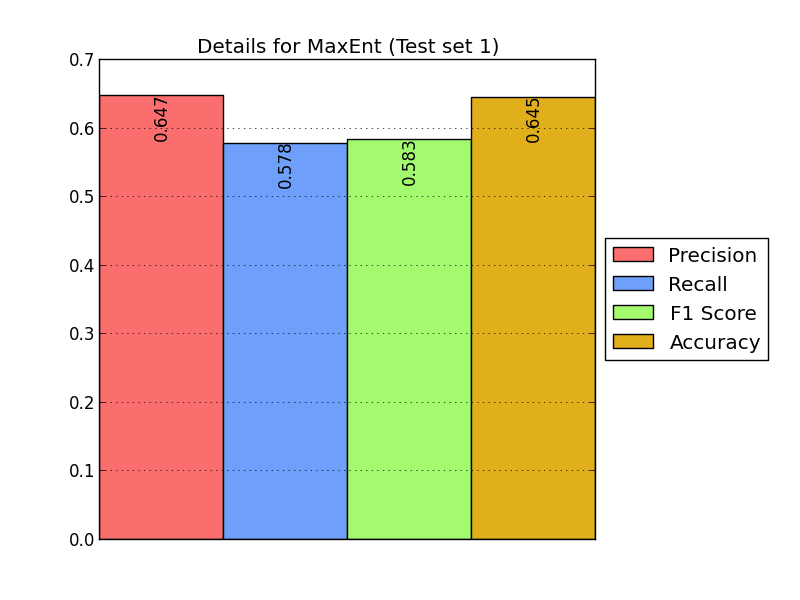
\includegraphics[width=\linewidth]{../img/plots/analysis/maxent_stats_best.png}
	\end{minipage}
	\hspace{0.05\linewidth}
	\begin{minipage}{.45\linewidth}
		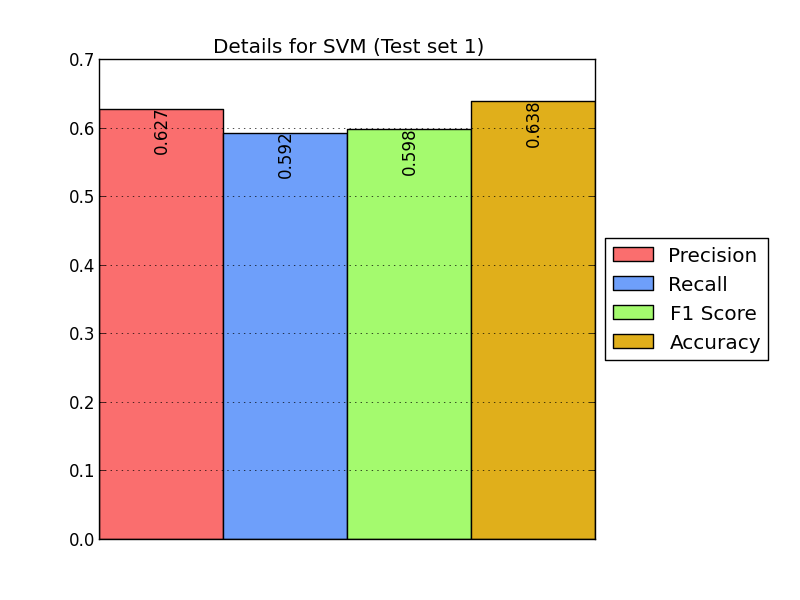
\includegraphics[width=\linewidth]{../img/plots/analysis/svm_stats_best.png}
	\end{minipage}
	\caption[Best performance plots for SVM and MaxEnt]{Best performance plots for SVM and MaxEnt. MaxEnt has better Precision and Accuracy, but SVM scores higher on F1-score and Recall.}
	\label{fig:best_result}
\end{figure}

\begin{figure}[t!]
	\centering
	\begin{minipage}{.45\linewidth}
		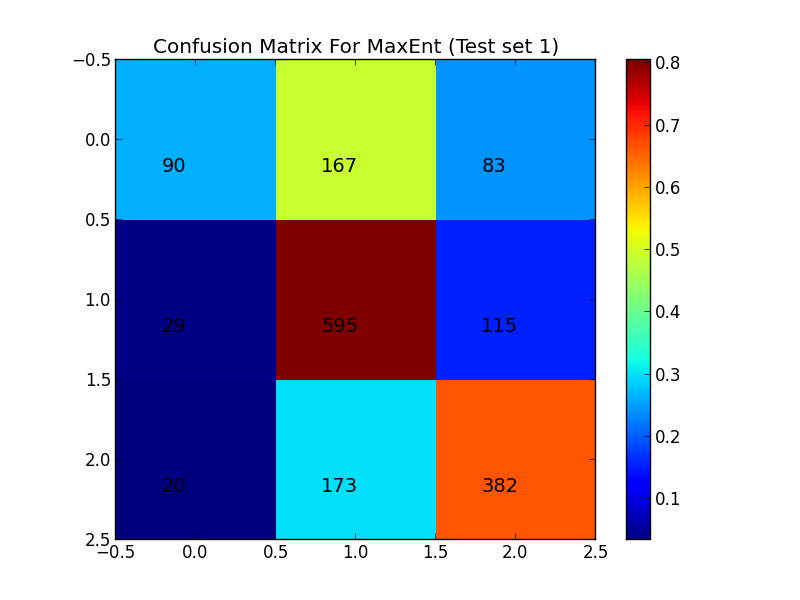
\includegraphics[width=\linewidth]{../img/plots/analysis/maxent_confusion_matrix_best.png}
	\end{minipage}
	\hspace{0.05\linewidth}
	\begin{minipage}{.45\linewidth}
		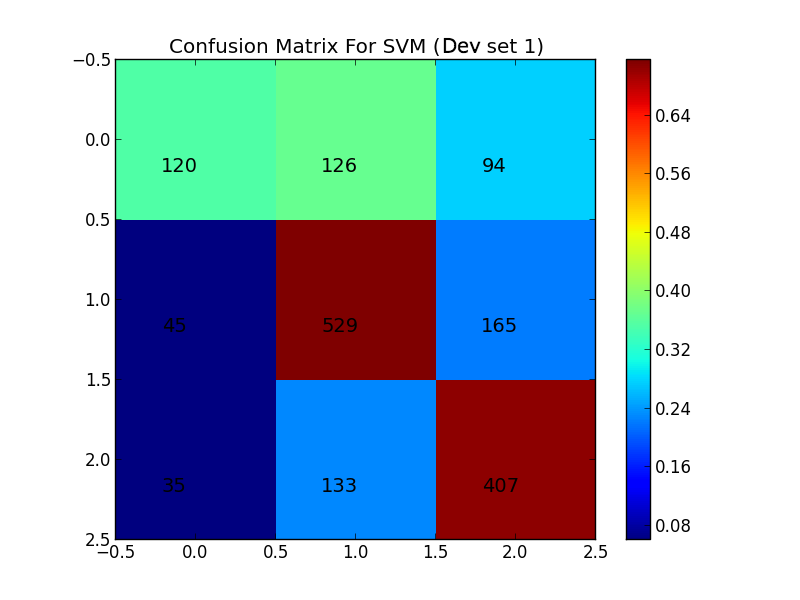
\includegraphics[width=\linewidth]{../img/plots/analysis/svm_confusion_matrix_best.png}
	\end{minipage}
	\caption[Confusion Matrix for SVM and MaxEnt]{Confusion Matrix for SVM and MaxEnt. MaxEnt favours neutral classification, and performs worse than SVM on both positive and negative classifications.}
	\label{fig:best_result_confusion}
\end{figure}

\begin{table}[t!]
	\centering
	\begin{tabular}{l|cc|cc} 
	\noalign{\smallskip}\hline\noalign{\smallskip}
	Data set & \multicolumn{2}{c|}{Dev set 1} & \multicolumn{2}{c}{Dev set 2} \\
	Learner  & SVM    & MaxEnt & SVM    & MaxEnt \\
	\noalign{\smallskip}\hline\noalign{\smallskip}
	Precision  & 0.627  & {\bf 0.647}   & {\bf 0.700}  & 0.561 \\
	Recall       & {\bf 0.592}  & 0.578  & {\bf 0.726}  & 0.589 \\
	F1-score  & {\bf 0.598}  & 0.583  & {\bf 0.707}  & 0.556 \\
	Accuracy & 0.638  & {\bf 0.645}  & {\bf 0.728}  & 0.581 \\
	\noalign{\smallskip}\hline\noalign{\smallskip}
	\end{tabular}
	\caption[Best classifier performance]{Best classifier performance {\small (bold=best score)}. Shows that using Dev 1, MaxEnt has better accuracy and precision, but SVM performs better in regards to F1-score and recall. For Dev 2, SVM has higher measures across the board.}
	\label{tab:performance}
\end{table}

\begin{figure}[t!]
	\centering
	\begin{minipage}{.45\linewidth}
		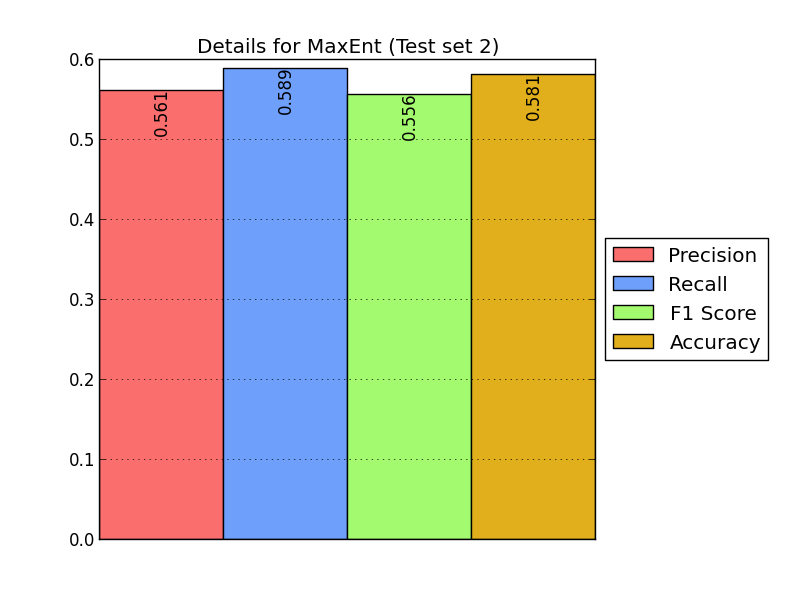
\includegraphics[width=\linewidth]{../img/plots/analysis/maxent_stats_best_diff_test.png}
	\end{minipage}
	\hspace{0.05\linewidth}
	\begin{minipage}{.45\linewidth}
		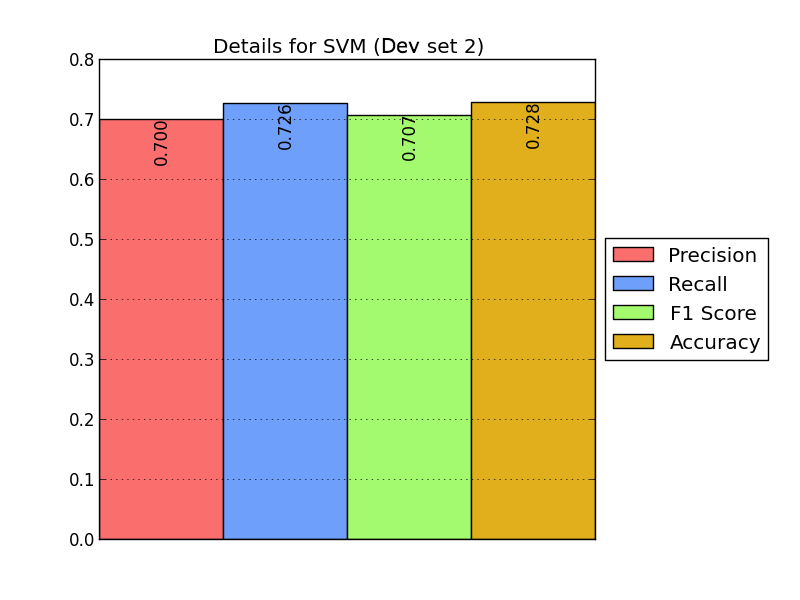
\includegraphics[width=\linewidth]{../img/plots/analysis/svm_stats_best_diff_test.png}
	\end{minipage}
	\caption[Best performance plots for SVM and MaxEnt for dev set 2]{Best performance plots for SVM and MaxEnt using Dev 2. SVM outperforms MaxEnt with \textbf{0.728} in accuracy versus \textbf{0.581}. SVM performs better according to all measures.}
	\label{fig:best_result_testset2}
\end{figure}

\begin{figure}[t!]
	\centering
	\begin{minipage}{.45\linewidth}
		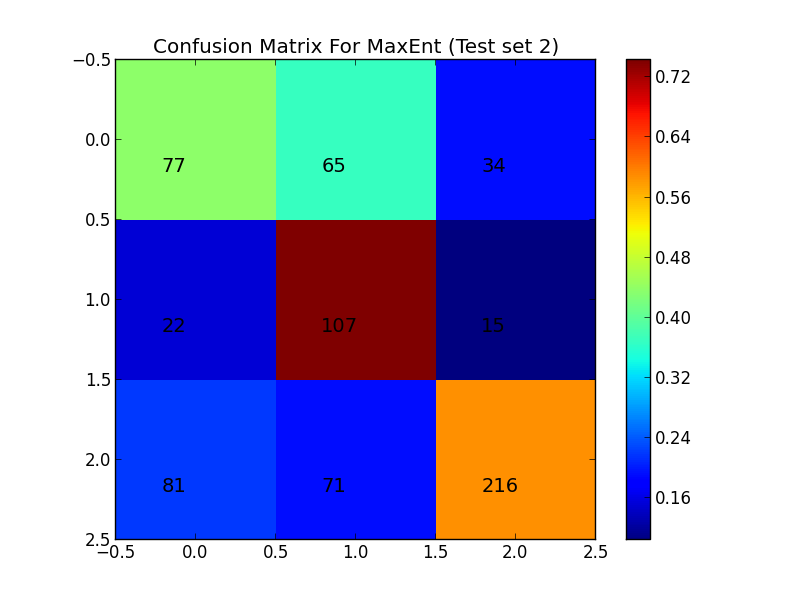
\includegraphics[width=\linewidth]{../img/plots/analysis/maxent_confusion_matrix_best_diff_test.png}
	\end{minipage}
	\hspace{0.05\linewidth}
	\begin{minipage}{.45\linewidth}
		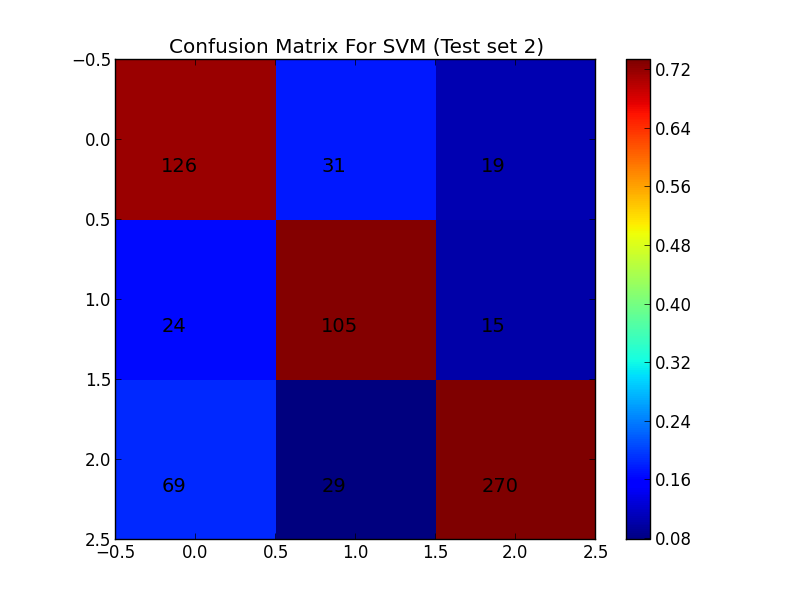
\includegraphics[width=\linewidth]{../img/plots/analysis/svm_confusion_matrix_best_diff_test.png}
	\end{minipage}
	\caption[Confusion Matrix for MaxEnt and SVM using dev set 2]{Confusion Matrix for MaxEnt and  using dev set 2. The performance difference between SVM and MaxEnt is visible in the confusion matrices as well. SVM shows a solid diagonal colour.}
	\label{fig:best_result_confusion_testset2}
\end{figure}

\begin{table}[t!]
	\centering
	\begin{tabular}{l|ccc} 
	\noalign{\smallskip}\hline\noalign{\smallskip}
	Data size  & Original       & 2000   & 1000 \\
	\noalign{\smallskip}\hline\noalign{\smallskip}
	Precision  & {\bf 0.627}  & 0.612 & 0.570 \\
	Recall       & 0.592  & \textbf{0.618} & 0.586 \\
	F1-score  & 0.598  & \textbf{0.614} & 0.563 \\
	Accuracy & {\bf 0.639}  & 0.630 & 0.569 \\
	\noalign{\smallskip}\hline\noalign{\smallskip}
	\end{tabular}
	\caption{Effects on SVM trained with reduced training sets}
	\label{tab:svm_reduced}
\end{table}

To even out the distribution of the different classes, we did a grid search with a reduced training set. Figure~\ref{fig:svm_reduced_1000} and~\ref{fig:svm_reduced_2000} show SVM's results when reducing the training set to a maximum of 1000 and 2000 tweets per class. The accuracy of SVM is highest on the original training set, but the F1-score and Recall improves when reducing the training set to maximum 2000 per class. See complete effects of reducing training set in~table~\ref{tab:svm_reduced}. The negative classification improves when reducing the training set to maximum 2000 tweets per class, but the accuracy for neutral and positive tweets decrease. Similar observation can be made when reducing the data set to 1000. Negative tweets perform better, but positive and neutral performance are worse. This can be deduced from~figures~\ref{fig:best_result_confusion},~\ref{fig:svm_reduced_2000} and~\ref{fig:svm_reduced_1000}.

\begin{figure}[t!]
	\centering
	\begin{minipage}{.45\linewidth}
		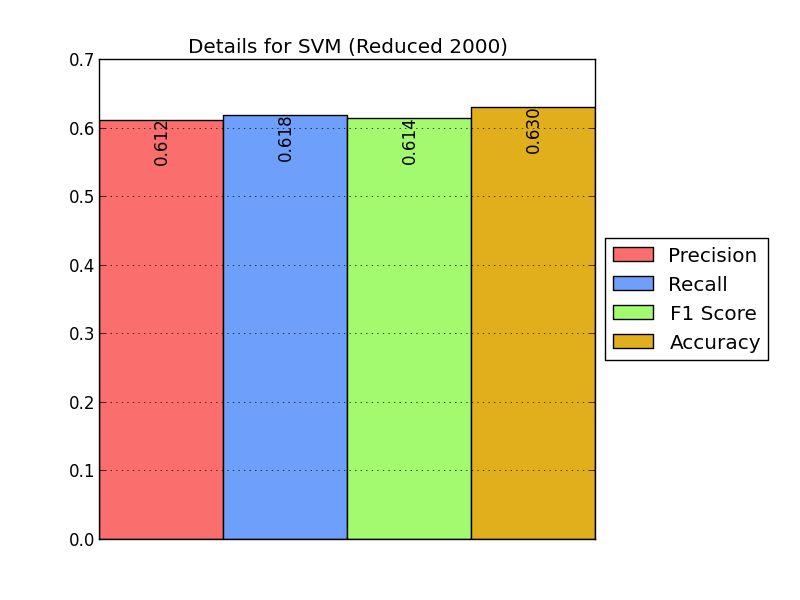
\includegraphics[width=\linewidth]{../img/plots/analysis/svm_stats_best_reduced_2000.png}
	\end{minipage}
	\hspace{0.05\linewidth}
	\begin{minipage}{.45\linewidth}
		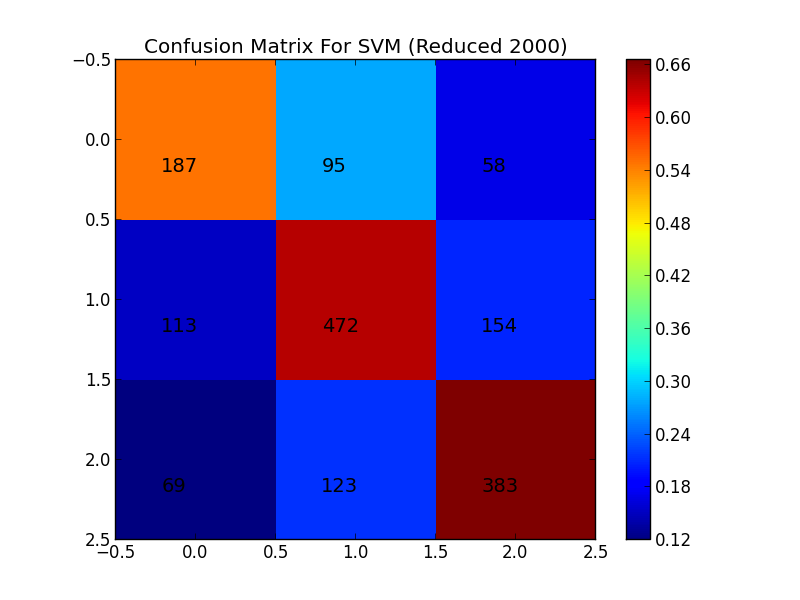
\includegraphics[width=\linewidth]{../img/plots/analysis/svm_confusion_matrix_best_reduced_2000.png}
	\end{minipage}
	\caption[Performance of SVM when reducing the dataset to max 2000 per class]{Performance of SVM when reducing the dataset to maximum 2000 per class. Showing better recall and F1-Score than without reduction, but poorer accuracy and precision. Somewhat better performance on negative tweets, but poorer on neutral and positive.}
	\label{fig:svm_reduced_2000}
\end{figure}

\begin{figure}[t!]
	\centering
	\begin{minipage}{.45\linewidth}
		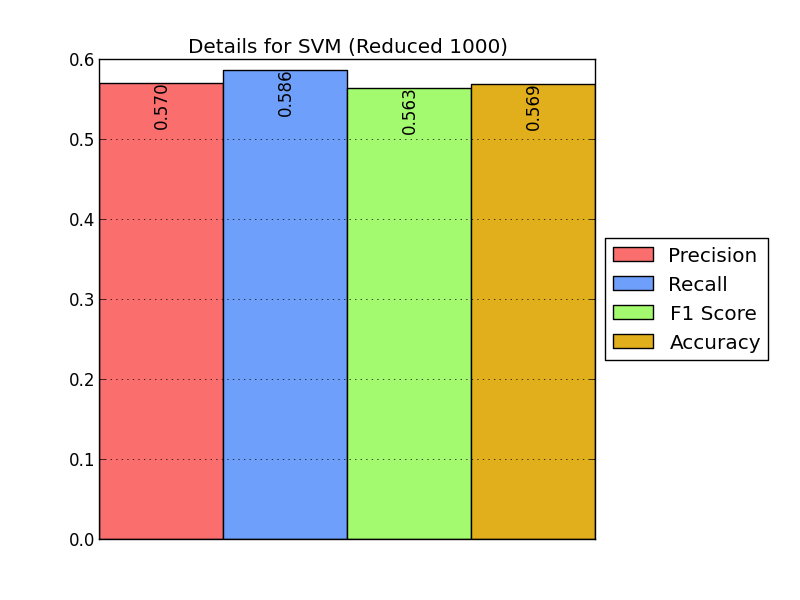
\includegraphics[width=\linewidth]{../img/plots/analysis/svm_stats_best_reduced_1000.png}
	\end{minipage}
	\hspace{0.05\linewidth}
	\begin{minipage}{.45\linewidth}
		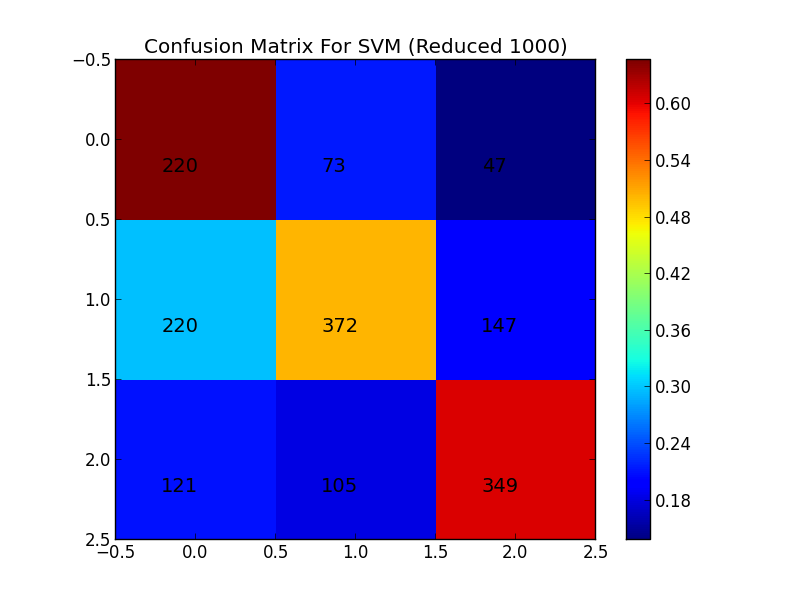
\includegraphics[width=\linewidth]{../img/plots/analysis/svm_confusion_matrix_best_reduced_1000.png}
	\end{minipage}
	\caption[Performance of SVM when reducing the dataset to max 1000 per class]{Performance of SVM when reducing the dataset to maximum 1000 per class. Showing better performance on negative tweets, but worse on neutral and positive. Performance is generally poorer than without reduction.}
	\label{fig:svm_reduced_1000}
\end{figure}

\begin{table}[t!]
\small
	\begin{minipage}{.45\linewidth}
		\begin{tabular}{|c|c|c|}
		
		\multicolumn{3}{c}{SVM} \\ \hline

		Negative & Neutral & Positive \\ \hline\hline

		no  		& wear & wait \\ \hline
		didn't  	& tallahassee & nice \\ \hline
		cancelled  	& 15th & interesting \\ \hline
		don't  		& 26 & awesome \\ \hline
		worse  		& at & cool \\ \hline
		why  		& trip & amazing \\ \hline
		bad  		& joe & fun \\ \hline
		worst  		& theres & ! \\ \hline
		hate  		& arrows & :) \\ \hline
		shit  		& murphy, & excited \\ \hline
		sad  		& question & happy \\ \hline
		sorry  		& plan & love \\ \hline
		not  		& set & best \\ \hline
		fuck  		& 8th & great \\ \hline
		:(  		& paterno & good \\ \hline
		\end{tabular}
	\end{minipage}
	\hspace{0.05\linewidth}
	\begin{minipage}{.45\linewidth}
		\begin{tabular}{|c|c|c|}		
		\multicolumn{3}{c}{MaxEnt} \\ \hline

		Negative & Neutral & Positive \\ \hline\hline

		no 	& center & glad \\ \hline
		don't 	& royal & nice \\ \hline
		why 	& plan & thanks \\ \hline
		bad 	& joe & cool \\ \hline
		shit 	& nov & awesome \\ \hline
		injury 	& george & interesting \\ \hline
		cancelled 	& theres & amazing \\ \hline
		hate 	& arrows & :) \\ \hline
		worst 	& trip & fun \\ \hline
		worse 	& set & best \\ \hline
		fuck 	& question & excited \\ \hline
		sorry 	& at & love \\ \hline
		not 	& url & happy \\ \hline
		sad 	& 8th & good \\ \hline
		:( 	& paterno & great \\ \hline
		\end{tabular}
	\end{minipage}
	\caption[Most informative features]{Top 15 of the most informative features for SVM and MaxEnt}
	\label{tab:informative_features}
\end{table}

The features in table~\ref{tab:informative_features} are the most informative features from each of the classifiers in the second grid search. Some features are represented among the top 15 for both SVM and MaxEnt, and most of these features make sense. As we did not normalize the features, we can see that some words appear in different forms and degrees (e.g., "worse", "worst" and "don't", "didn't"). For both MaxEnt and SVM, emoticons are listed among the most informative features. In the case of SVM, the exclamation mark is an informative feature for positive classification.

We see that for the most part the features seem to make sense, but we see some anomalies. Both SVM and MaxEnt show 'why' as a negative feature, which is normally incorrect. In addition, the most informative positive feature for SVM is 'wait', which is not a particularly positively charged word.

\clearpage
\section{SemEval'13 Results}~\label{sec:semeval_result}

Based on the information from the grid search, two systems were built for SemEval'13. Since one-step SVM-based classification showed the best performance on the training data, it was chosen for the system participating in the constrained subtask, NTNUC. The pre-processing was also the one with the best performance on the provided data, P2 which involves lower-casing all letters; reducing letter duplicates; using hash-tags as words (removing \#); and removing all URLs, user names and RT -tags.

\begin{table}[t!]

\centering
\begin{tabular}{l|cc|cc} 
\noalign{\smallskip}\hline\noalign{\smallskip}
	& \multicolumn{2}{c|}{Twitter}	& \multicolumn{2}{c}{SMS} \\
 \multicolumn{1}{r|}{\bf NTNU-}	&  {\footnotesize NTNUC}	& {\footnotesize NTNUU}	& {\footnotesize NTNUC}	& {\footnotesize NTNUU} \\
\noalign{\smallskip}\hline\noalign{\smallskip}
Precision    				& {\bf 0.652}	& 0.633 	& {\bf 0.659} 	& 0.623 \\
Recall       				& {\bf 0.579}  	& 0.564 	& {\bf 0.646} 	& 0.623  \\
F1-score  				& {\bf 0.590}  	& 0.572 	& {\bf 0.652} 	& 0.623  \\
F1 pos/neg 				& {\bf 0.532}  	& 0.507 	& {\bf 0.580} 	& 0.546  \\
\noalign{\smallskip}\hline\noalign{\smallskip}
\end{tabular}

\caption{{\bf NTNUC} and {\bf NTNUU} in SemEval'13}
\label{tab:semeval_results}
\end{table}

Given the small size of the in-house ('NTNU') data set, no major improvement was expected from adding it in the unconstrained task. Instead, a radically different set-up was chosen to create a new system, and train it on both the in-house and provided data. NTNUU utilizes a two-step approach, with SVM for subjectivity and MaxEnt for polarity classification, a combination intended to capture the strengths of both algorithms. No preprocessing was used for the subjectivity step, but user names were removed before attempting polarity classification.

As further described by~\citet{WilsonEA:13}, the SemEval'13 shared task involved testing on a set of 3813 tweets (1572 positive, 601 negative, and 1640 neutral). In order to evaluate classification performance on data of roughly the same length and type, but from a different domain, the evaluation data also included 2094 Short Message Service texts (SMS; 492 positive, 394 negative, and 1208 neutral).

Table \ref{tab:semeval_results}~shows the results obtained by the NTNU systems on the SemEval'13 evaluation data, in terms of average precision, recall and F-score for all three classes, as well as average F-score for positive and negative tweets only (F1 + / \textendash; i.e., the measure used to rank the systems participating in the shared task).

THe NTNU system ranked at 24th of 36 on constrained and 10th of 15 on unconstrained. For the SMS task, the NTNU system ranked 5th of 28 constrained systems and 6th of 15 unconstrained.


\section{Visualisation Results}~\label{sec:esc_result}

During the experiment a screen shot of the SentiStack system was taken to document the results (see~figure~\ref{fig:sentistack_esc}).

\begin{figure}[htb!]
	\centering
	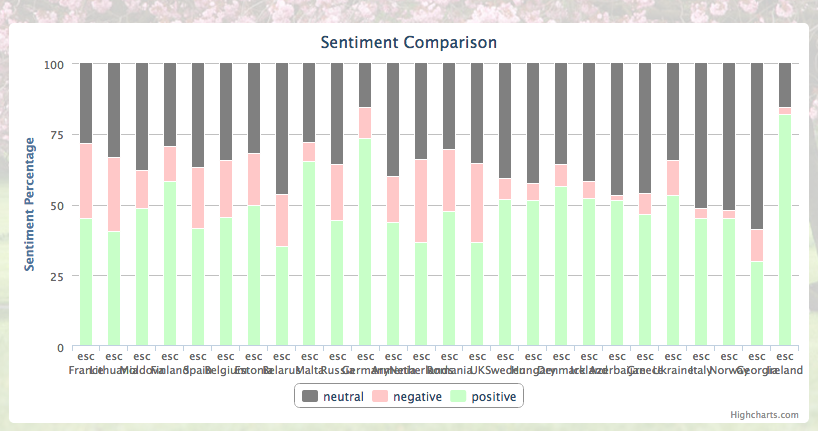
\includegraphics[width=\linewidth]{../img/sentistack_esc.png}
	\caption[SentiStack running before the Eurovision Song Contest Final]{The SentiStack application running before the Eurovision Song Contest Final. The order of the bar stacks is equal to the running order: France, Lithuania, Moldova, Finland, Spain, Belgium, Estonia, Belarus, Malta, Russia, Germany, Armenia, The Netherlands, Romania, United Kingdom, Sweden, Hungary, Denmark, Iceland, Azerbaijan, Greece, Ukraine, Italy, Norway, Georgia and Ireland.}
	\label{fig:sentistack_esc}
\end{figure}

The application was run before the final, but after the semi-finals. The goal was to predict as much of the top-10 list as possible. By sheer guesswork, one could expect to get $\dfrac{10}{26} = 0.3846 \approx 38.5\%$\footnote{10 out of 26 participants.} of the top-10 finalists. 

In figure~\ref{fig:sentistack_esc}, the prediction results is shown. By the graph, it is clearly visible that Ireland was predicted to be the winner, followed by Germany, Malta, Finland and Denmark.

Table~\ref{tab:esc_results} shows an overview of the predictions and the actual results of the ESC 2013. Only 5 of the predicted top-10 actually resulted amongst the top-10; thus the system had an accuracy of 50\%. 

\begin{table}

\centering
\begin{tabular}{|c|l|l|} 
\hline
 Place	&  Prediction	& Result  \\ \hline \hline

1. & Ireland & \textbf{Denmark}      \\ \hline
2. & Germany & \textbf{Azerbaijan}   \\ \hline
3. & \textbf{Malta} & \textbf{Ukraine}      \\ \hline
4. & Finland & Norway       \\ \hline
5. & \textbf{Denmark} & Russia       \\ \hline
6. & \textbf{Ukraine} & Greece       \\ \hline
7. & Iceland & Italy        \\ \hline
8. & Sweden & \textbf{Malta}        \\ \hline
9. & \textbf{Hungary} & Netherlands  \\ \hline
10. & \textbf{Azerbaijan} & \textbf{Hungary}  \\ \hline

\end{tabular}

\caption[Eurovision Song Contest experiment result]{The results of the Eurovision Song Contest versus the predictions from using the SentiStack visualisation application. From the table, it is visible that 50\% of the countries predicted in the top-10, resulted in a position among the top-10. The countries shared between the lists are marked in bold.}
\label{tab:esc_results}
\end{table}

%
%\subsubsection{SentiMap After a Natural Disaster}
%
%\begin{figure}[htb!]
%	\centering
%	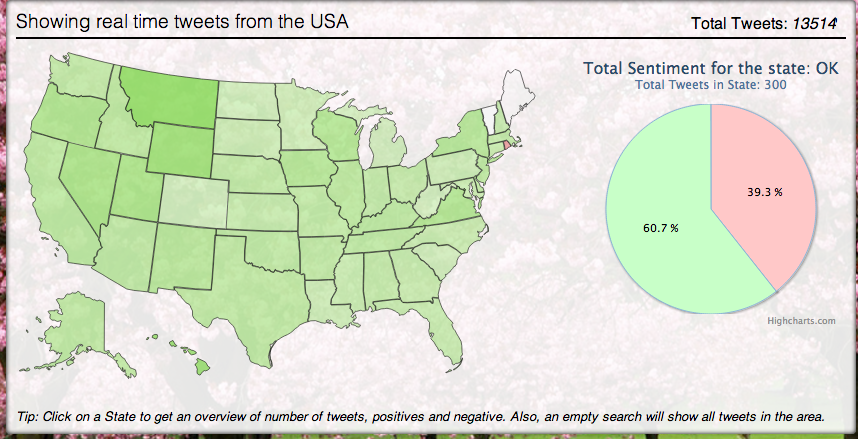
\includegraphics[width=\linewidth]{../img/disaster_sentimap.png}
%	\caption[SentiMap after a natural disaster]{Showing SentiMap running after a natural disaster in Oklahoma. Showing little change in sentiment in the state or the nation. Positive tweets at 60.7\%.}
%	\label{fig:disaster_sentimap}
%\end{figure}
%
%There was no notable change in sentiment for Oklahoma over time after the tornado disaster. After streaming tweets for a while, the sentiment normalized at 60.7\% positive and 39.4\% negative. This is about the same as previous runs. This is shown in~figure~\ref{fig:disaster_sentimap}. 
%
%Results from searching on Oklahoma on SentiGraph show that many tweets related to 
%
%\begin{figure}[htb!]
%	\centering
%	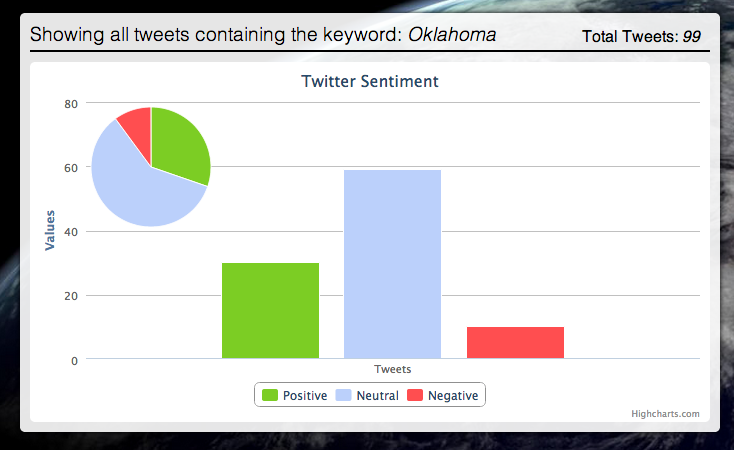
\includegraphics[width=\linewidth]{../img/disaster_graph.png}
%	\caption[SentiGraph plots after a natural disaster]{SentiGraph after a natural disaster in Oklahoma. Showing a large portion of the tweets as neutral and many positive.}
%	\label{fig:disaster_graph}
%\end{figure}
%
%
%
%\begin{figure}[htb!]
%	\centering
%	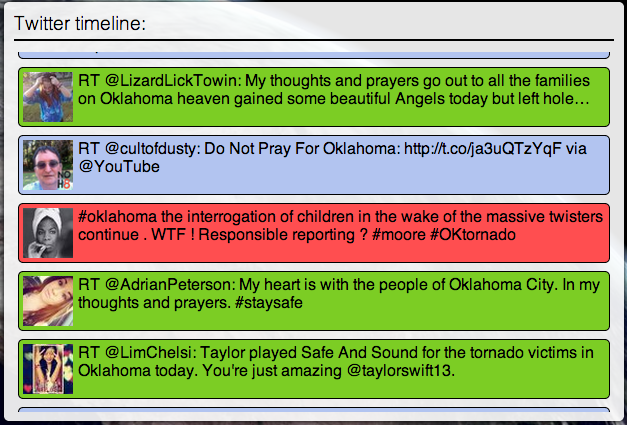
\includegraphics[width=\linewidth]{../img/disaster_list.png}
%	\caption[SentiGraph tweet list after a natural disaster]{SentiGraph showing tweets after a natural disaster in Oklahoma. Many tweets classified as positive with prayers for Oklahoma, and many neutral tweets with links to different news sites and articles.}
%	\label{fig:disaster_list}
%\end{figure}